\documentclass[12pt]{article}

\usepackage[letterpaper,margin=1in]{geometry}
\usepackage[colorlinks,linkcolor=blue,urlcolor=magenta]{hyperref}
\usepackage{amsmath,tikz,xparse,graphicx,mathtools,mathdots,chngcntr}

\input{/home/loppy/latex/lib/sets.tex}
\input{/home/loppy/latex/lib/vector.tex}
\input{/home/loppy/latex/lib/algebra.tex}
\input{/home/loppy/latex/lib/brackets.tex}

\renewcommand\thepart{\arabic{part}}
\numberwithin{section}{part}
\numberwithin{equation}{section}

\newcommand\s{\hphantom-}
\newcommand\n{\hphantom1}
\newcommand\numberthis{\stepcounter{equation}\tag\theequation}
\newcommand\mm[1]{\mathbf{#1}}
\newcommand\m[2]{\text{#1$#2$}}
\newcommand\mLarge[1]{\m\Large{#1}}
\newcommand\topstrut[1]{\rule{0pt}{#1}}
\newcommand\one{\m\large{\mathbf{1}}}

\NewDocumentCommand\trans{s m}{%
  \IfBooleanTF{#1}%
    {\left(#2\right)^{\!\!\top}}%
    {#2^{\top}}%
}

\DeclareMathOperator\Isom{Isom}
\newcommand\Cube{\ensuremath{\mathcal C}}
\newcommand\IsomC{\ensuremath{\Isom(\Cube)}}

\title{Isometries of the Cube}
\author{Nicholas Todoroff}
\date\today

\begin{document}
\maketitle

\vspace{-5mm}
{\centering\emph{[Note: This document is not complete]}\par}
\vspace{-5mm}
\part*{Introduction}
                           This paper is divided into two parts.

Part~\ref{part:construction} is a short, sweet, and direct construction of all isometries
\IsomC\ of the cube as matrices over $\R^3$.

Part~\ref{part:generators}

Part~\ref{part:adjrep}

\part{Constuction}
  \label{part:construction}\stepcounter{section}
Let the cube \Cube\ be represented by its eight vertices $\vv y_1, \vv y_2, \dotsc, \vv y_8 \in
\R^3$ where
\begin{align*}
\vv y_1 &= (\s1, \s1, \s1),\quad \vv y_2 = (\s1, -1, \s1),\quad \vv y_3 = (-1, -1, \s1),\quad
  \vv y_4 = (-1, \s1, \s1),\quad \\
\vv y_5 &= (-1, \s1, -1),\quad \vv y_6 = (-1, -1, -1),\quad \vv y_7 = (\s1, -1, -1),\quad
  \vv y_8 = (\s1, \s1, -1). \numberthis\label{eqn:verts}
\end{align*}
We can easily determine the order $|\IsomC|$, since it must preserve which vertices neighbor
which. First, choose one of the eight vertices. Then, there are exactly three other vertices
that it must be connected to, which we may choose from and place beside it. Finally, there are
two vertices that may be placed beside this, since it is already beside the originally chosen
vertex. The number of isometries must then be
\[ |\IsomC| = 8\cdot3\cdot2 = 48. \]

Each face of \Cube\ may be represented by a standard basis vector or its negative
\[
\pm\unitv x_1 = (\pm1, 0, 0),\quad \pm\unitv x_2 = (0, \pm1, 0),\quad
\pm\unitv x_3 = (0, 0, \pm1).
\]
In particular, it will be useful in Section~\ref{sec:adj->R3} to know that
\begin{equation}\label{eqn:vert-to-face}
\unitv x_1 = \frac14(\vv y_1+\vv y_2+\vv y_7+\vv y_8),\quad
\unitv x_2 = \frac14(\vv y_1+\vv y_4+\vv y_5+\vv y_8),\quad
\unitv x_3 = \frac14(\vv y_1+\vv y_2+\vv y_3+\vv y_4).
\end{equation}
Any $M \in \IsomC$ must map faces to faces, and so must map $\pm\unitv x_j \mapsto \pm\unitv
x_k$ for some $j, k = 1, 2, 3$. $M$ is also invertible since $\vv v \mapsto M\vv v$ is
one-to-one by definition of \IsomC, and so its' columns must be linearly independent. This
forces the columns of $M$ to take the form
\begin{equation}\label{eqn:isommat}
M = (\pm\unitv x_a, \pm\unitv x_b, \pm\unitv x_c)
\end{equation}
where $(a, b, c)$ is a permutation of $(1, 2, 3)$. There are $3!$ permutations and $2^3$
choices of sign, making
\[ 3!\cdot2^3 = 48 \]
such matrices, so this necessarily characterizes all $M \in \IsomC$.

\part{Generators}
  \label{part:generators}  Number the vertices of \Cube\ in accordance with Eq.~\ref{eqn:verts}:
\begin{center}
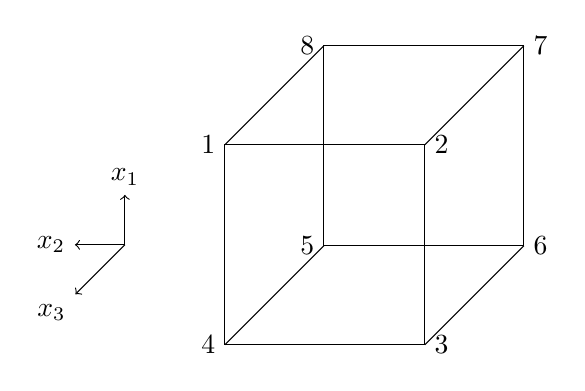
\begin{tikzpicture}
\draw (0,0)      -- ++(0,1in) -- ++(-1in,0) -- ++(0,-1in) -- ++(1in,0);
\draw (45:0.7in) -- ++(0,1in) -- ++(-1in,0) -- ++(0,-1in) -- ++(1in,0);
\draw (0,0)      node[anchor=west]{3} -- ++(45:0.7in) node[anchor=west]{6};
\draw (0,1in)    node[anchor=west]{2} -- ++(45:0.7in) node[anchor=west]{7};
\draw (-1in,1in) node[anchor=east]{1} -- ++(45:0.7in) node[anchor=east]{8};
\draw (-1in,0)   node[anchor=east]{4} -- ++(45:0.7in) node[anchor=east]{5};

\draw[->] (-1.5in,0.5in) -- ++(0,0.25in)    node[anchor=south]{$\unitv x_1$};
\draw[->] (-1.5in,0.5in) -- ++(-0.25in,0)   node[anchor=east]{$\unitv x_2$};
\draw[->] (-1.5in,0.5in) -- ++(-135:0.35in) node[anchor=north east]{$\unitv x_3$};
\end{tikzpicture}
\end{center}
All isometries of \Cube\ may be formed from three generators, here written as permutations
of the vertices:
\begin{equation}\label{eqn:gens}
R = (1234)(8765),\quad r = (12)(34)(56)(78),\quad s = (135)(268).
\end{equation}

\section{Proof of Generation}     $R$ is the rotation of the $x_3$-face; $r$ is the reflection in the $x_1x_3$-plane; and $s$ is
the rotation ("spin") that holds 4 and 7 fixed. It is easy to see, from visualization or
computation, that the orders of these elements are
\[ |\gen R| = 4,\quad |\gen{r_1}| = |\gen{r_2}| = 2,\quad |\gen s| = 3. \]
To show that these are indeed generators, it will be useful to consider the reflections
$r_{12}$ and $r_{23}$ about the respective $x_1x_2$-, $x_2x_3$-planes (noting that
$r=r_{13}$), as well as the rotations $R_1, R_2, R_3$ about the respective $x_1$-, $x_2$-,
$x_3$-axes (noting that $R = R_3^{-1}$). We see that
\begin{alignat*}3
srs^{-1} &= (36)(54)(18)(72) = r_{12},\quad & RrR^{-1}     &= (23)(41)(85)(67) = r_{23}, \\
sRs^{-1} &= (3654)(2781) = R_1,\quad        & s^{2}Rs^{-2} &= (5814)(6723) = R_2^{-1}.
  \numberthis\label{eqn:gen->sp}
\end{alignat*}
So these elements (and their inverses) are in $\gen{R,r,s}$. Consider now the $\R^3$
representations of $r_{12}, r_{23}, r_{13}, R_1, R_2, R_3$, which are easily obtainable by
considering the transformation of the faces of \Cube:
\begin{alignat*}3
 r_{12} &\mapsto \begin{pmatrix}\s1 &\s0 &\s0\s \\\s0 &\s1 &\s0\s \\\s0 &\s0 & -1\s \end{pmatrix},\quad
&r_{23} &\mapsto \begin{pmatrix} -1 &\s0 &\s0\s \\\s0 &\s1 &\s0\s \\\s0 &\s0 &\s1\s \end{pmatrix},\quad
&r_{13} &\mapsto \begin{pmatrix}\s1 &\s0 &\s0\s \\\s0 & -1 &\s0\s \\\s0 &\s0 &\s1\s \end{pmatrix}, \\
 R_1    &\mapsto \begin{pmatrix}\s1 &\s0 &\s0\s \\\s0 &\s0 &\s1\s \\\s0 & -1 &\s0\s \end{pmatrix},\quad
&R_2    &\mapsto \begin{pmatrix}\s0 &\s0 & -1\s \\\s1 &\s0 &\s0\s \\\s0 &\s1 &\s0\s \end{pmatrix},\quad
&R_3    &\mapsto \begin{pmatrix}\s0 &\s1 &\s0\s \\ -1 &\s0 &\s0\s \\\s0 &\s0 &\s1\s \end{pmatrix}.
\end{alignat*}
In particular, it is easiest to study the combinations
\begin{subequations}\label{eqn:sp-mat}
\begin{alignat*}6
 r_{12}    &\mapsto \begin{pmatrix}\s1 &\s0 &\s0\s \\\s0 &\s1 &\s0\s \\\s0 &\s0 & -1\s \end{pmatrix},\quad
&r_{23}    &\mapsto \begin{pmatrix} -1 &\s0 &\s0\s \\\s0 &\s1 &\s0\s \\\s0 &\s0 &\s1\s \end{pmatrix},\quad
&r_{13}    &\mapsto \begin{pmatrix}\s1 &\s0 &\s0\s \\\s0 & -1 &\s0\s \\\s0 &\s0 &\s1\s \end{pmatrix}, \numberthis\label{eqn:s-mat} \\
 r_{12}R_1 &\mapsto \begin{pmatrix}\s1 &\s0 &\s0\s \\\s0 &\s0 &\s1\s \\\s0 &\s1 &\s0\s \end{pmatrix},\quad
&r_{23}R_2 &\mapsto \begin{pmatrix}\s0 &\s0 &\s1\s \\\s1 &\s0 &\s0\s \\\s0 &\s1 &\s0\s \end{pmatrix},\quad
&rR_3      &\mapsto \begin{pmatrix}\s0 &\s1 &\s0\s \\\s1 &\s0 &\s0\s \\\s0 &\s0 &\s1\s \end{pmatrix}. \numberthis\label{eqn:p-mat}
\end{alignat*}
\end{subequations}
The matrices of $r_{12}R_1, r_{23}R_2, r_{13}R_3$ are precisely the standard permutation matrices
of $(23), (123), (12)$, respectively, and generate all six possible permutation matrices:
\[
(1),\quad (12),\quad (23),\quad
\underbrace{(13)}_{=(12)(23)},\quad
(123),\quad
\underbrace{(321)}_{=(12)(123)}. \]
It was shown in Part~\ref{part:construction} that all elements of $M \in \IsomC$ are of the
form (Eq.~\ref{eqn:isommat})
\[ M = (\pm\unitv x_a, \pm\unitv x_b, \pm\unitv x_c) \]
for some permutation $(a, b, c)$ of $(1, 2, 3)$ and choice of signs, and that each choice of
permutation and sign corresponds to a unique element of \IsomC. The elements
Eq.~\ref{eqn:s-mat} allow us to choose the sign, and the elements Eq.~\ref{eqn:p-mat} allow us
to choose the permutation. Given a choice of sign $\iota = (\iota_1, \iota_2, \iota_3)$ and
permutaton $\sigma \in S_3$, we can now build every element $M^\iota_\sigma \in \IsomC$ as
\begin{equation}\label{eqn:sp-rep}
M^\iota_\sigma = m(\sigma)r_{23}^{n(\iota_1)}r_{13}^{n(\iota_2)}r_{12}^{n(\iota_3)}
               = r_{23}^{n(\iota_{\sigma(1)})}r_{13}^{n(\iota_{\sigma(2)})}r_{12}^{n(\iota_{\sigma(3)})}m(\sigma),
\end{equation}
where
\begin{gather*}
n(x) = \frac{1-x}2, \\
\begin{aligned}
m((1))\n &= 1,\quad                  & m((12))\n &= r_{13}R_3,\quad            & m((23))\n &= r_{12}R_1,\quad \\
m((13))  &= r_{12}R_1r_{13}R_3,\quad & m((123))  &= r_{23}R_2,\quad & m((321)) &= r_{13}R_3r_{23}R_2.
\end{aligned}
\end{gather*}
It is thus that $\gen{R, r, s} = \IsomC$.

\subsection*{Aside}
The second equality in Eq.~\ref{eqn:sp-rep} comes from the fact that right multiplication by
e.g. $r_{23}$ sets the sign of the first \emph{column} of $m(\sigma)$, and left multiplication
sets the sign of the first \emph{row}. Each row and column of $m(\sigma)$ contains exactly one
1, and the map that links corresponding rows and columns is exactly $\sigma$.

It is clear that $\gen{r_{23}, r_{13}, r_{12}}$ and the set of permutation matrices $P_3 =
\set{m(\sigma)}[\sigma \in S_3] \iso S_3$ are trivially intersecting subgroups of \IsomC. This
second equality then shows us that $\gen{r_{23}, r_{13}, r_{12}}$ is a normal subgroup of
\IsomC, and it follows that
\[ \quot{\IsomC}{\gen{r_{23}, r_{13}, r_{12}}} \iso S_3. \]
Of course, this is not surprising since we've already shown that \IsomC\ is the set of signed
permutation matrices. Note however that this does not mean that \IsomC\ is a product group:
\[ \IsomC \not\iso C_2^3\times S_3, \]
where $C_2^3 \iso \gen{r_{23}, r_{13}, r_{12}}$ is the product of three order-two cyclic
groups. While Eq.~\ref{eqn:sp-rep} does tell us that $\gen{r_{23}, r_{13}, r_{12}}$ is normal,
it also explicitly shows that it does not commute with $P_3$.


\part{Adjacency Representation}
  \label{part:adjrep}      Number the vertices of \Cube\ in accordance with Eq.~\ref{eqn:verts}:
\begin{center}
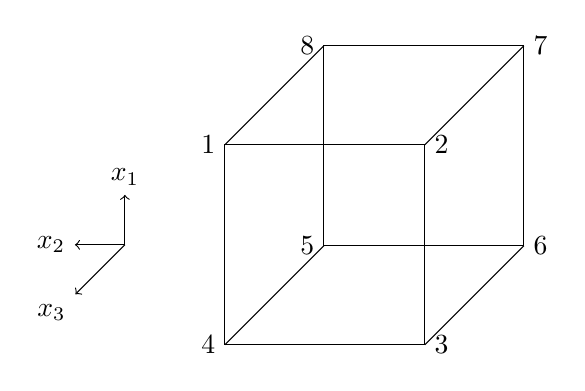
\begin{tikzpicture}
\draw (0,0)      -- ++(0,1in) -- ++(-1in,0) -- ++(0,-1in) -- ++(1in,0);
\draw (45:0.7in) -- ++(0,1in) -- ++(-1in,0) -- ++(0,-1in) -- ++(1in,0);
\draw (0,0)      node[anchor=west]{3} -- ++(45:0.7in) node[anchor=west]{6};
\draw (0,1in)    node[anchor=west]{2} -- ++(45:0.7in) node[anchor=west]{7};
\draw (-1in,1in) node[anchor=east]{1} -- ++(45:0.7in) node[anchor=east]{8};
\draw (-1in,0)   node[anchor=east]{4} -- ++(45:0.7in) node[anchor=east]{5};

\draw[->] (-1.5in,0.5in) -- ++(0,0.25in)    node[anchor=south]{$\unitv x_1$};
\draw[->] (-1.5in,0.5in) -- ++(-0.25in,0)   node[anchor=east]{$\unitv x_2$};
\draw[->] (-1.5in,0.5in) -- ++(-135:0.35in) node[anchor=north east]{$\unitv x_3$};
\end{tikzpicture}
\end{center}
All isometries of \Cube\ may be formed from three generators, here written as permutations
of the vertices:
\begin{equation}\label{eqn:gens}
R = (1234)(8765),\quad r = (12)(34)(56)(78),\quad s = (135)(268).
\end{equation}

\section{Proof of Generation}     $R$ is the rotation of the $x_3$-face; $r$ is the reflection in the $x_1x_3$-plane; and $s$ is
the rotation ("spin") that holds 4 and 7 fixed. It is easy to see, from visualization or
computation, that the orders of these elements are
\[ |\gen R| = 4,\quad |\gen{r_1}| = |\gen{r_2}| = 2,\quad |\gen s| = 3. \]
To show that these are indeed generators, it will be useful to consider the reflections
$r_{12}$ and $r_{23}$ about the respective $x_1x_2$-, $x_2x_3$-planes (noting that
$r=r_{13}$), as well as the rotations $R_1, R_2, R_3$ about the respective $x_1$-, $x_2$-,
$x_3$-axes (noting that $R = R_3^{-1}$). We see that
\begin{alignat*}3
srs^{-1} &= (36)(54)(18)(72) = r_{12},\quad & RrR^{-1}     &= (23)(41)(85)(67) = r_{23}, \\
sRs^{-1} &= (3654)(2781) = R_1,\quad        & s^{2}Rs^{-2} &= (5814)(6723) = R_2^{-1}.
  \numberthis\label{eqn:gen->sp}
\end{alignat*}
So these elements (and their inverses) are in $\gen{R,r,s}$. Consider now the $\R^3$
representations of $r_{12}, r_{23}, r_{13}, R_1, R_2, R_3$, which are easily obtainable by
considering the transformation of the faces of \Cube:
\begin{alignat*}3
 r_{12} &\mapsto \begin{pmatrix}\s1 &\s0 &\s0\s \\\s0 &\s1 &\s0\s \\\s0 &\s0 & -1\s \end{pmatrix},\quad
&r_{23} &\mapsto \begin{pmatrix} -1 &\s0 &\s0\s \\\s0 &\s1 &\s0\s \\\s0 &\s0 &\s1\s \end{pmatrix},\quad
&r_{13} &\mapsto \begin{pmatrix}\s1 &\s0 &\s0\s \\\s0 & -1 &\s0\s \\\s0 &\s0 &\s1\s \end{pmatrix}, \\
 R_1    &\mapsto \begin{pmatrix}\s1 &\s0 &\s0\s \\\s0 &\s0 &\s1\s \\\s0 & -1 &\s0\s \end{pmatrix},\quad
&R_2    &\mapsto \begin{pmatrix}\s0 &\s0 & -1\s \\\s1 &\s0 &\s0\s \\\s0 &\s1 &\s0\s \end{pmatrix},\quad
&R_3    &\mapsto \begin{pmatrix}\s0 &\s1 &\s0\s \\ -1 &\s0 &\s0\s \\\s0 &\s0 &\s1\s \end{pmatrix}.
\end{alignat*}
In particular, it is easiest to study the combinations
\begin{subequations}\label{eqn:sp-mat}
\begin{alignat*}6
 r_{12}    &\mapsto \begin{pmatrix}\s1 &\s0 &\s0\s \\\s0 &\s1 &\s0\s \\\s0 &\s0 & -1\s \end{pmatrix},\quad
&r_{23}    &\mapsto \begin{pmatrix} -1 &\s0 &\s0\s \\\s0 &\s1 &\s0\s \\\s0 &\s0 &\s1\s \end{pmatrix},\quad
&r_{13}    &\mapsto \begin{pmatrix}\s1 &\s0 &\s0\s \\\s0 & -1 &\s0\s \\\s0 &\s0 &\s1\s \end{pmatrix}, \numberthis\label{eqn:s-mat} \\
 r_{12}R_1 &\mapsto \begin{pmatrix}\s1 &\s0 &\s0\s \\\s0 &\s0 &\s1\s \\\s0 &\s1 &\s0\s \end{pmatrix},\quad
&r_{23}R_2 &\mapsto \begin{pmatrix}\s0 &\s0 &\s1\s \\\s1 &\s0 &\s0\s \\\s0 &\s1 &\s0\s \end{pmatrix},\quad
&rR_3      &\mapsto \begin{pmatrix}\s0 &\s1 &\s0\s \\\s1 &\s0 &\s0\s \\\s0 &\s0 &\s1\s \end{pmatrix}. \numberthis\label{eqn:p-mat}
\end{alignat*}
\end{subequations}
The matrices of $r_{12}R_1, r_{23}R_2, r_{13}R_3$ are precisely the standard permutation matrices
of $(23), (123), (12)$, respectively, and generate all six possible permutation matrices:
\[
(1),\quad (12),\quad (23),\quad
\underbrace{(13)}_{=(12)(23)},\quad
(123),\quad
\underbrace{(321)}_{=(12)(123)}. \]
It was shown in Part~\ref{part:construction} that all elements of $M \in \IsomC$ are of the
form (Eq.~\ref{eqn:isommat})
\[ M = (\pm\unitv x_a, \pm\unitv x_b, \pm\unitv x_c) \]
for some permutation $(a, b, c)$ of $(1, 2, 3)$ and choice of signs, and that each choice of
permutation and sign corresponds to a unique element of \IsomC. The elements
Eq.~\ref{eqn:s-mat} allow us to choose the sign, and the elements Eq.~\ref{eqn:p-mat} allow us
to choose the permutation. Given a choice of sign $\iota = (\iota_1, \iota_2, \iota_3)$ and
permutaton $\sigma \in S_3$, we can now build every element $M^\iota_\sigma \in \IsomC$ as
\begin{equation}\label{eqn:sp-rep}
M^\iota_\sigma = m(\sigma)r_{23}^{n(\iota_1)}r_{13}^{n(\iota_2)}r_{12}^{n(\iota_3)}
               = r_{23}^{n(\iota_{\sigma(1)})}r_{13}^{n(\iota_{\sigma(2)})}r_{12}^{n(\iota_{\sigma(3)})}m(\sigma),
\end{equation}
where
\begin{gather*}
n(x) = \frac{1-x}2, \\
\begin{aligned}
m((1))\n &= 1,\quad                  & m((12))\n &= r_{13}R_3,\quad            & m((23))\n &= r_{12}R_1,\quad \\
m((13))  &= r_{12}R_1r_{13}R_3,\quad & m((123))  &= r_{23}R_2,\quad & m((321)) &= r_{13}R_3r_{23}R_2.
\end{aligned}
\end{gather*}
It is thus that $\gen{R, r, s} = \IsomC$.

\subsection*{Aside}
The second equality in Eq.~\ref{eqn:sp-rep} comes from the fact that right multiplication by
e.g. $r_{23}$ sets the sign of the first \emph{column} of $m(\sigma)$, and left multiplication
sets the sign of the first \emph{row}. Each row and column of $m(\sigma)$ contains exactly one
1, and the map that links corresponding rows and columns is exactly $\sigma$.

It is clear that $\gen{r_{23}, r_{13}, r_{12}}$ and the set of permutation matrices $P_3 =
\set{m(\sigma)}[\sigma \in S_3] \iso S_3$ are trivially intersecting subgroups of \IsomC. This
second equality then shows us that $\gen{r_{23}, r_{13}, r_{12}}$ is a normal subgroup of
\IsomC, and it follows that
\[ \quot{\IsomC}{\gen{r_{23}, r_{13}, r_{12}}} \iso S_3. \]
Of course, this is not surprising since we've already shown that \IsomC\ is the set of signed
permutation matrices. Note however that this does not mean that \IsomC\ is a product group:
\[ \IsomC \not\iso C_2^3\times S_3, \]
where $C_2^3 \iso \gen{r_{23}, r_{13}, r_{12}}$ is the product of three order-two cyclic
groups. While Eq.~\ref{eqn:sp-rep} does tell us that $\gen{r_{23}, r_{13}, r_{12}}$ is normal,
it also explicitly shows that it does not commute with $P_3$.



\newpage
\part*{Appendix}
                           Number the vertices of \Cube\ in accordance with Eq.~\ref{eqn:verts}:
\begin{center}
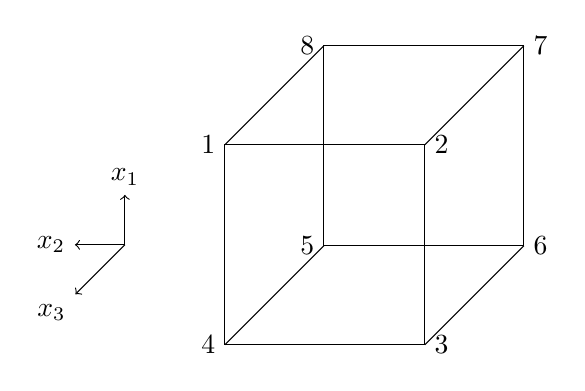
\begin{tikzpicture}
\draw (0,0)      -- ++(0,1in) -- ++(-1in,0) -- ++(0,-1in) -- ++(1in,0);
\draw (45:0.7in) -- ++(0,1in) -- ++(-1in,0) -- ++(0,-1in) -- ++(1in,0);
\draw (0,0)      node[anchor=west]{3} -- ++(45:0.7in) node[anchor=west]{6};
\draw (0,1in)    node[anchor=west]{2} -- ++(45:0.7in) node[anchor=west]{7};
\draw (-1in,1in) node[anchor=east]{1} -- ++(45:0.7in) node[anchor=east]{8};
\draw (-1in,0)   node[anchor=east]{4} -- ++(45:0.7in) node[anchor=east]{5};

\draw[->] (-1.5in,0.5in) -- ++(0,0.25in)    node[anchor=south]{$\unitv x_1$};
\draw[->] (-1.5in,0.5in) -- ++(-0.25in,0)   node[anchor=east]{$\unitv x_2$};
\draw[->] (-1.5in,0.5in) -- ++(-135:0.35in) node[anchor=north east]{$\unitv x_3$};
\end{tikzpicture}
\end{center}
All isometries of \Cube\ may be formed from three generators, here written as permutations
of the vertices:
\begin{equation}\label{eqn:gens}
R = (1234)(8765),\quad r = (12)(34)(56)(78),\quad s = (135)(268).
\end{equation}

\section{Proof of Generation}     $R$ is the rotation of the $x_3$-face; $r$ is the reflection in the $x_1x_3$-plane; and $s$ is
the rotation ("spin") that holds 4 and 7 fixed. It is easy to see, from visualization or
computation, that the orders of these elements are
\[ |\gen R| = 4,\quad |\gen{r_1}| = |\gen{r_2}| = 2,\quad |\gen s| = 3. \]
To show that these are indeed generators, it will be useful to consider the reflections
$r_{12}$ and $r_{23}$ about the respective $x_1x_2$-, $x_2x_3$-planes (noting that
$r=r_{13}$), as well as the rotations $R_1, R_2, R_3$ about the respective $x_1$-, $x_2$-,
$x_3$-axes (noting that $R = R_3^{-1}$). We see that
\begin{alignat*}3
srs^{-1} &= (36)(54)(18)(72) = r_{12},\quad & RrR^{-1}     &= (23)(41)(85)(67) = r_{23}, \\
sRs^{-1} &= (3654)(2781) = R_1,\quad        & s^{2}Rs^{-2} &= (5814)(6723) = R_2^{-1}.
  \numberthis\label{eqn:gen->sp}
\end{alignat*}
So these elements (and their inverses) are in $\gen{R,r,s}$. Consider now the $\R^3$
representations of $r_{12}, r_{23}, r_{13}, R_1, R_2, R_3$, which are easily obtainable by
considering the transformation of the faces of \Cube:
\begin{alignat*}3
 r_{12} &\mapsto \begin{pmatrix}\s1 &\s0 &\s0\s \\\s0 &\s1 &\s0\s \\\s0 &\s0 & -1\s \end{pmatrix},\quad
&r_{23} &\mapsto \begin{pmatrix} -1 &\s0 &\s0\s \\\s0 &\s1 &\s0\s \\\s0 &\s0 &\s1\s \end{pmatrix},\quad
&r_{13} &\mapsto \begin{pmatrix}\s1 &\s0 &\s0\s \\\s0 & -1 &\s0\s \\\s0 &\s0 &\s1\s \end{pmatrix}, \\
 R_1    &\mapsto \begin{pmatrix}\s1 &\s0 &\s0\s \\\s0 &\s0 &\s1\s \\\s0 & -1 &\s0\s \end{pmatrix},\quad
&R_2    &\mapsto \begin{pmatrix}\s0 &\s0 & -1\s \\\s1 &\s0 &\s0\s \\\s0 &\s1 &\s0\s \end{pmatrix},\quad
&R_3    &\mapsto \begin{pmatrix}\s0 &\s1 &\s0\s \\ -1 &\s0 &\s0\s \\\s0 &\s0 &\s1\s \end{pmatrix}.
\end{alignat*}
In particular, it is easiest to study the combinations
\begin{subequations}\label{eqn:sp-mat}
\begin{alignat*}6
 r_{12}    &\mapsto \begin{pmatrix}\s1 &\s0 &\s0\s \\\s0 &\s1 &\s0\s \\\s0 &\s0 & -1\s \end{pmatrix},\quad
&r_{23}    &\mapsto \begin{pmatrix} -1 &\s0 &\s0\s \\\s0 &\s1 &\s0\s \\\s0 &\s0 &\s1\s \end{pmatrix},\quad
&r_{13}    &\mapsto \begin{pmatrix}\s1 &\s0 &\s0\s \\\s0 & -1 &\s0\s \\\s0 &\s0 &\s1\s \end{pmatrix}, \numberthis\label{eqn:s-mat} \\
 r_{12}R_1 &\mapsto \begin{pmatrix}\s1 &\s0 &\s0\s \\\s0 &\s0 &\s1\s \\\s0 &\s1 &\s0\s \end{pmatrix},\quad
&r_{23}R_2 &\mapsto \begin{pmatrix}\s0 &\s0 &\s1\s \\\s1 &\s0 &\s0\s \\\s0 &\s1 &\s0\s \end{pmatrix},\quad
&rR_3      &\mapsto \begin{pmatrix}\s0 &\s1 &\s0\s \\\s1 &\s0 &\s0\s \\\s0 &\s0 &\s1\s \end{pmatrix}. \numberthis\label{eqn:p-mat}
\end{alignat*}
\end{subequations}
The matrices of $r_{12}R_1, r_{23}R_2, r_{13}R_3$ are precisely the standard permutation matrices
of $(23), (123), (12)$, respectively, and generate all six possible permutation matrices:
\[
(1),\quad (12),\quad (23),\quad
\underbrace{(13)}_{=(12)(23)},\quad
(123),\quad
\underbrace{(321)}_{=(12)(123)}. \]
It was shown in Part~\ref{part:construction} that all elements of $M \in \IsomC$ are of the
form (Eq.~\ref{eqn:isommat})
\[ M = (\pm\unitv x_a, \pm\unitv x_b, \pm\unitv x_c) \]
for some permutation $(a, b, c)$ of $(1, 2, 3)$ and choice of signs, and that each choice of
permutation and sign corresponds to a unique element of \IsomC. The elements
Eq.~\ref{eqn:s-mat} allow us to choose the sign, and the elements Eq.~\ref{eqn:p-mat} allow us
to choose the permutation. Given a choice of sign $\iota = (\iota_1, \iota_2, \iota_3)$ and
permutaton $\sigma \in S_3$, we can now build every element $M^\iota_\sigma \in \IsomC$ as
\begin{equation}\label{eqn:sp-rep}
M^\iota_\sigma = m(\sigma)r_{23}^{n(\iota_1)}r_{13}^{n(\iota_2)}r_{12}^{n(\iota_3)}
               = r_{23}^{n(\iota_{\sigma(1)})}r_{13}^{n(\iota_{\sigma(2)})}r_{12}^{n(\iota_{\sigma(3)})}m(\sigma),
\end{equation}
where
\begin{gather*}
n(x) = \frac{1-x}2, \\
\begin{aligned}
m((1))\n &= 1,\quad                  & m((12))\n &= r_{13}R_3,\quad            & m((23))\n &= r_{12}R_1,\quad \\
m((13))  &= r_{12}R_1r_{13}R_3,\quad & m((123))  &= r_{23}R_2,\quad & m((321)) &= r_{13}R_3r_{23}R_2.
\end{aligned}
\end{gather*}
It is thus that $\gen{R, r, s} = \IsomC$.

\subsection*{Aside}
The second equality in Eq.~\ref{eqn:sp-rep} comes from the fact that right multiplication by
e.g. $r_{23}$ sets the sign of the first \emph{column} of $m(\sigma)$, and left multiplication
sets the sign of the first \emph{row}. Each row and column of $m(\sigma)$ contains exactly one
1, and the map that links corresponding rows and columns is exactly $\sigma$.

It is clear that $\gen{r_{23}, r_{13}, r_{12}}$ and the set of permutation matrices $P_3 =
\set{m(\sigma)}[\sigma \in S_3] \iso S_3$ are trivially intersecting subgroups of \IsomC. This
second equality then shows us that $\gen{r_{23}, r_{13}, r_{12}}$ is a normal subgroup of
\IsomC, and it follows that
\[ \quot{\IsomC}{\gen{r_{23}, r_{13}, r_{12}}} \iso S_3. \]
Of course, this is not surprising since we've already shown that \IsomC\ is the set of signed
permutation matrices. Note however that this does not mean that \IsomC\ is a product group:
\[ \IsomC \not\iso C_2^3\times S_3, \]
where $C_2^3 \iso \gen{r_{23}, r_{13}, r_{12}}$ is the product of three order-two cyclic
groups. While Eq.~\ref{eqn:sp-rep} does tell us that $\gen{r_{23}, r_{13}, r_{12}}$ is normal,
it also explicitly shows that it does not commute with $P_3$.


\end{document}
